\documentclass[11pt]{article}
\usepackage[a4paper,margin=28mm]{geometry}
\usepackage{amsmath,amssymb,amsthm,mathtools,booktabs}
\usepackage[T1]{fontenc}
\usepackage{lmodern,microtype}
\usepackage{tikz}
\usetikzlibrary{arrows.meta,positioning}
\usepackage{xurl}
\usepackage[hidelinks]{hyperref}
\newtheorem{theorem}{Theorem}[section]
\newtheorem{lemma}[theorem]{Lemma}
\newtheorem{proposition}[theorem]{Proposition}
\newtheorem{corollary}[theorem]{Corollary}
\theoremstyle{remark}\newtheorem{remark}[theorem]{Remark}
\newcommand{\R}{\mathbb R}
\newcommand{\C}{\mathbb C}
\newcommand{\Z}{\mathbb Z}
\newcommand{\spec}{\operatorname{spec}}
\newcommand{\diag}{\operatorname{diag}}
\newcommand{\tr}{\operatorname{tr}}
\newcommand{\norm}[1]{\left\lVert#1\right\rVert}
\newcommand{\rstar}{r_*}
\newcommand{\tw}{\rho_{\mathrm{tw}}}
\newcommand{\cone}{c_1}
\newcommand{\czero}{c_0}
\newcommand{\etaedge}{\eta_*}
\title{Uniform Schur bounds for unequal cells in signed cycle squares}
\author{}
\date{Revised research manuscript\quad 5 October 2026}
\begin{document}
\maketitle
\begin{abstract}
We prove spectral bounds for explicit signed cycle squares built from an
arbitrary positive number of unequal prescribed cells. A four-dimensional
Riccati recurrence with exact rational premises gives a common
six-dimensional limiting boundary matrix, whose degree-two assembly error
is independent of the number of cells. For either Hamilton holonomy,
the construction satisfies a squared spectral-radius bound of
$7.92$ when every cell has length at least $106$, and $7.90537$ when every
cell has length at least $202$. The one-cell family satisfies the
sharper bound at every admissible size, and its supremum lies in an interval
of width $10^{-6}$. Exact finite bases complete explicit competitors to the
twisted signing at orders $32,40$ and every even order at least $48$.
This recovers the previously known witness range through a common analytic
mechanism. We also present the exact period-eight holonomy calculation and
its application to the revised global-optimality conjecture. Unrestricted
minima and minimizing signings are not determined.
\end{abstract}
\section{Introduction and main results}

For $N\ge8$, the cycle square $C_N(1,2)$ has vertex set $\Z/N\Z$ and
edges $\{i,i+1\}$ and $\{i,i+2\}$. A real signing assigns $\pm1$ to each
edge. For its symmetric adjacency matrix $A$, write
\[
 \rho(A)=\max\{|\lambda|:\lambda\in\spec(A)\},
 \qquad \mu_N=\min_\sigma\rho(A_\sigma).
\]
The minimization controls both spectral edges. The benchmark in the
original twisted-optimality question \cite{Suvagiya2026old} is
\begin{equation}
 \tw(N)^2=4+2\cos\frac{2\pi}{N}+2\cos\frac{4\pi}{N}
 \qquad(N\text{ even},\ N\ge8).
 \label{eq:twisted}
\end{equation}

We seek an explicit family whose spectral bound survives two changes at
once: its cells may have different lengths, and their number is unrestricted.
A fixed-period calculation alone does not cover this setting. Our main
result follows by eliminating each cell interior, retaining its boundary
coordinates, and controlling the assembled cyclic boundary matrix with an
error independent of the number of cells. The cells are built from the
period-eight word
\begin{equation}
 t=(1,1,-1,1,-1,-1,1,-1),\qquad
 w_j=t^j\mathbin{\|}(1,-1),\qquad h_j=8j+2\quad(j\ge1).
 \label{eq:word}
\end{equation}
Here $\|$ denotes concatenation. Appending $(1,-1)$ adds two vertices to
the period-eight bulk, so that $r$ such cells give order $2r$ modulo eight.
In the associated quadrilateral signs $Q_u=\tau_u\tau_{u+1}$, the positive
positions are separated by four within a cell and by six across a boundary.
Thus the prescribed cells insert one length-six gap per cell into the
length-four pattern, while retaining arbitrarily long period-eight stretches.
The precise words, rather than the gap count alone, are the hypotheses.

For a length-$N$ triangle-sign word
$\tau$ and $\alpha\in\{\pm1\}$, define $A_N(\tau,\alpha)$ by the edge signs
\begin{equation}
 a_i=\begin{cases}1&i<N-1,\\\alpha&i=N-1,\end{cases}
 \quad
 \sigma\{i,i+1\}=a_i,\qquad
 \sigma\{i,i+2\}=\tau_i a_i a_{i+1},
 \label{eq:gauge-definition}
\end{equation}
with cyclic indices. The triangle signs are $\tau_i$, and the
Hamilton-cycle sign product is $\alpha$.
The two rational caps below are certified upper thresholds for these
constructions, rather than proposed values of the unrestricted minimum:
define
\[
 \czero=\frac{198}{25}=7.92,\qquad
 \cone=\frac{790537}{100000}=7.90537.
\]

\begin{theorem}[Unequal-cell bound]\label{thm:cells}
Let $r\ge1$, $j_0,\ldots,j_{r-1}\ge1$, and
$\tau=w_{j_0}\|\cdots\|w_{j_{r-1}}$, of total length $N$.
For either holonomy $\alpha$,
\begin{align}
 \min_i h_{j_i}\ge106&\quad\Longrightarrow\quad
       \rho(A_N(\tau,\alpha))^2<\czero,\label{eq:cell-cap0}\\
 \min_i h_{j_i}\ge202&\quad\Longrightarrow\quad
       \rho(A_N(\tau,\alpha))^2<\cone.\label{eq:cell-cap1}
\end{align}
The constants do not depend on $r$, and the lengths need not be equal.
\end{theorem}

The allowed cell words are part of the hypotheses. The theorem does not
cover arbitrary signings or arbitrary arrangements of local defects.
Its proof retains six coordinates at each cell boundary and eliminates the
four-site interior chains exactly. A common positive limiting core and a
quadratic-form estimate with two chain incidences per boundary control the
resulting $6r$-dimensional cyclic matrix. The two chain incidences at every boundary, rather than the total number
of cells, determine the error estimate.

The single-cell family permits a sharper finite completion.
\begin{theorem}[One-cell bound]\label{thm:one-cell}
For every $k\ge1$,
\[
 \rho(A_{8k+2}(w_k,+1))^2<\cone.
\]
Moreover,
\begin{equation}
 \frac{7905369}{1000000}
 <\sup_{k\ge1}\rho(A_{8k+2}(w_k,+1))^2
 \le\frac{790537}{100000}.
 \label{eq:supremum}
\end{equation}
\end{theorem}
The interval in \eqref{eq:supremum} has width $10^{-6}$. Its upper endpoint
is non-strict; no convergence, monotonicity, or exact supremum is asserted.

To cover each nonzero even residue modulo eight, put
\[
 W_{k,r}=\mathop{\|}_{a=0}^{r-1}w_{\lfloor(k+a)/r\rfloor},
 \qquad r\in\{1,2,3\},\ k\ge6.
\]
The cell parameters sum to $k$, so the word has length $8k+2r$.
\begin{theorem}[Explicit finite competitors]\label{thm:witnesses}
For $r\in\{1,2,3\}$ and $k\ge6$, the matrix
\[
 B_{k,r}=A_{8k+2r}(W_{k,r},(-1)^{r+1})
\]
satisfies
\begin{equation}
 \rho(B_{k,r})^2<\czero<\tw(8k+2r)^2.
 \label{eq:nonzero-witnesses}
\end{equation}
For $r=1$ the stronger cap $\cone$ holds. Together with the period-eight
family, these constructions prove
\[
 \mu_N<\tw(N)
 \quad\text{for }N\in\{32,40\}\cup\{N\ge48:N\text{ even}\}.
\]
\end{theorem}

The period-eight predecessor \cite{EarlierPeriodEight} already supplies the
orders $32$ and $40$, and the earlier Target A package
\cite{EarlierTargetA} supplies every even order at least $48$.
These are unpublished project predecessors. The contribution here is a
common analytic mechanism, sharper quantitative bounds, and a finite
completion with directly specified signings. For odd $k$ in residue four, and for
$3\nmid k$ in residue six, our placements need not be the older balanced-gap
placements. Their finite certificates are recomputed for the words above.
We do not reprove the universal lower bounds at complementary smaller
orders, determine $\mu_N$ when the twisted signing fails, or classify
minimizing signings.

The literature target has also changed. The original preprint
\cite{Suvagiya2026old} was withdrawn and merged into
\cite{Suvagiya2026}. Its revised Theorem 26 supplies the positive-holonomy
period-eight value
\begin{equation}
 \etaedge=4+\sqrt{10+2\sqrt5},\qquad \rstar=\sqrt{\etaedge},
 \label{eq:rstar}
\end{equation}
for $N=8m$, $m\ge4$, while Conjecture 28 proposes $\mu_{8m}=\rstar$
throughout that range. The exact negative-holonomy formula from the earlier
project manuscript \cite{EarlierPeriodEight} is strictly smaller at every
finite size. We provide its full proof and apply it to that revised claim.
This application is distinct from a priority claim for the inherited formula.

Schur complements and contractive Riccati recurrences are standard matrix
tools. The contribution here is their quantitative assembly for the stated
cells: a common limiting core controls unequal chains, and the retained
matrix has two chain incidences per boundary. Related signed-spectral
results concern different questions. Belardo and Brunetti
\cite[Theorem 1.3 and Lemma 3.8]{BelardoBrunetti2024} determine limit points
of signed adjacency spectral radii and use a Schur-complement calculation
for an auxiliary family. Our one-cell enclosure does not identify a new
limit point or prove convergence. Kannan and Pragada
\cite[Theorem 3.3]{KannanPragada2023} bound the largest adjacency eigenvalue
using edge count, frustration index, and balanced clique number. Here the
input is the prescribed triangle-sign word and its boundary response; the
result controls both spectral edges uniformly in cell length and count.

The use of holonomy belongs to the established character approach to
spectral graph theory; Luo and Roy \cite[Theorems 3.6 and 3.13]{LuoRoy2026}
study character families and endpoint attainment. Those results do not
supply the fixed-support minimum here. Likewise, signed moments averaged
over all signings, as in Chen, van Dam, and Bu
\cite[Theorem 3.1]{ChenDamBu2024}, are not pointwise lower bounds for every
signing. Our estimates instead arise from an explicit fiber calculation
and exact positive-definiteness tests after a uniform analytic reduction.
The latter proofs are finite-certificate-assisted, with independent exact
replays; their finite checks are specified in Section~\ref{sec:finite} and
located in the frozen supplement \cite{C029Supplement}.

The proof has two tracks. Sections~\ref{sec:holonomy}--\ref{sec:period8}
give the exact period-eight calculation and its application to the revised
conjecture; this track is independent of the Schur estimates.
Sections~\ref{sec:chain}--\ref{sec:cells} prove
Theorem~\ref{thm:cells}: positivity of $cI-A^2$ is reduced to a fixed
four-dimensional recurrence, two finite rational premise sets control its
tail, and the six-coordinate boundary matrices assemble with degree two.
Section~\ref{sec:finite} then completes the bounded ranges needed for the
one-cell specialization and the all-residue competitors.
Figure~\ref{fig:boundary} displays the local-to-global reduction.

\section{Switching and finite holonomy}\label{sec:holonomy}

Write $a_i$ for the sign of $\{i,i+1\}$ and $d_i$ for the sign of
$\{i,i+2\}$, with cyclic indices. The triangle sign and Hamilton-cycle
holonomy are
\[
 \tau_i=a_i a_{i+1}d_i,\qquad \alpha=\prod_{i=0}^{n-1}a_i.
\]
Switching by vertex signs $g_i\in\{\pm1\}$ replaces $A$ by $GAG$,
where $G=\diag(g_i)$. It preserves the spectrum, every $\tau_i$, and
$\alpha$.

\begin{lemma}\label{lem:gauge}
For prescribed triangle signs $(\tau_i)_{i\in\Z/n\Z}$, there are exactly
two switching classes, indexed by $\alpha\in\{\pm1\}$. Each has a unique
representative with
\[
 a_0=\cdots=a_{n-2}=1,\qquad a_{n-1}=\alpha,
 \qquad d_i=\tau_i a_i a_{i+1}.
\]
\end{lemma}
\begin{proof}
Set $g_0=1$ and recursively $g_{i+1}=g_i a_i$ for $0\le i<n-1$.
After switching, the first $n-1$ step-one signs are positive. Their product
with the remaining sign is $\alpha$, so that remaining sign is $\alpha$.
The triangle equations force every step-two sign. Conversely, the displayed
signs realize the prescribed data for either choice of $\alpha$.
A switch between two such representatives is constant along the path
$0,1,\ldots,n-1$, hence constant on all vertices and acts trivially.
Finally, distinct values of the switching invariant $\alpha$ cannot be
switching equivalent.
\end{proof}

For the repeated word $t^m$ on $N=8m$ vertices, write
$A_m^\pm=A_{8m}(t^m,\pm1)$. The positive representative has all step-one
signs positive and step-two signs $t_{i\bmod8}$. The negative representative
reverses exactly the three distinct edges
\begin{equation}
 \{N-1,0\},\qquad\{N-2,0\},\qquad\{N-1,1\}.
 \label{eq:seam}
\end{equation} Reversing only the Hamilton edge would
change two triangle signs. The two additional step-two reversals are
therefore essential.

Extend $u\in\C^{8m}$ to the integer line by
\begin{equation}
 u_{i+8m}=\alpha u_i.
 \label{eq:extension}
\end{equation}
Let $t_i=t_{i\bmod8}$. In either seam gauge the adjacency action is the
restriction of
\begin{equation}
 (Lu)_i=u_{i-1}+u_{i+1}+t_{i-2}u_{i-2}+t_i u_{i+2}.
 \label{eq:infinite-action}
\end{equation}
In particular, the signs of all cut-crossing edges in the finite matrix
agree with \eqref{eq:extension}, including for $m=1$.

\begin{lemma}\label{lem:bloch}
The complexification of $A_m^\alpha$ is unitarily equivalent to
\[
 \bigoplus_{z^m=\alpha}H(z),
\]
where, in the order $0,1,\ldots,7$,
\begin{equation}
 H(z)=\begin{pmatrix}
0&1&1&0&0&0&z^{-1}&z^{-1}\\
1&0&1&1&0&0&0&-z^{-1}\\
1&1&0&1&-1&0&0&0\\
0&1&1&0&1&1&0&0\\
0&0&-1&1&0&1&-1&0\\
0&0&0&1&1&0&1&-1\\
z&0&0&0&-1&1&0&1\\
z&-z&0&0&0&-1&1&0
\end{pmatrix}.
\label{eq:fiber}
\end{equation}
\end{lemma}
\begin{proof}
For each root $z^m=\alpha$ and $v\in\C^8$, set
$u_{8j+a}=m^{-1/2}z^jv_a$ for $0\le j<m$ and $0\le a<8$.
This satisfies \eqref{eq:extension}. Substitution into
\eqref{eq:infinite-action} gives \eqref{eq:fiber}. For two different
allowed phases $z,w$, the ratio $z\overline w$ is a nontrivial $m$th
root of unity, so
\[
 \sum_{j=0}^{m-1}(z\overline w)^j=0.
\]
Thus the $m$ fiber spaces are mutually orthogonal, each has dimension
eight, and together they exhaust dimension $8m$. The displayed map is
unitary. Since $|z|=1$, the fiber matrix is Hermitian.
\end{proof}

\section{The exact antiperiodic spectrum}\label{sec:period8}

Let $A_m^\pm=A_{8m}(t^m,\pm1)$ and set
\[
 R(s)=\sqrt{4+\sqrt{8+s+\sqrt{26-3s}}}\qquad(-2\le s\le2).
\]
\begin{theorem}\label{thm:period8}
For every $m\ge1$,
\begin{equation}
 \rho(A_m^+)^2=\etaedge,
 \qquad \rho(A_m^-)=R\!\left(2\cos\frac\pi m\right)<\sqrt{\etaedge}.
 \label{eq:main}
\end{equation}
Among signings with the prescribed labeled triangle signs $t^m$, the
negative-holonomy class is the unique minimizing switching class.
\end{theorem}
The exact formula is recorded in the earlier period-eight manuscript
\cite{EarlierPeriodEight}; we include its proof to keep the present
argument self-contained.

\begin{lemma}\label{lem:poly}
For $|z|=1$ and $s=z+z^{-1}$,
\begin{align}
 \det(xI_8-H(z))=P(x,s)
  &:=x^8-16x^6+80x^4-128x^2+38 \notag\\
  &\quad+s(-2x^4+16x^2-13)+s^2.
 \label{eq:poly}
\end{align}
Its eight roots, with all signs independently chosen, are
\begin{equation}
 \pm\sqrt{4\pm\sqrt{8+s\pm\sqrt{26-3s}}}.
 \label{eq:all-roots}
\end{equation}
They are all real, nonzero, and distinct for every $-2\le s\le2$.
\end{lemma}
\begin{proof}
Expanding the determinant of \eqref{eq:fiber} as a Laurent polynomial
in $z$ gives
\[
 x^8-16x^6+80x^4-128x^2+40
 +(z+z^{-1})(-2x^4+16x^2-13)+(z^2+z^{-2}).
\]
Using $z^2+z^{-2}=s^2-2$ proves \eqref{eq:poly}.
This is a finite polynomial identity and can also be checked by the exact
symbolic determinant in the accompanying verifier.

Put $y=x^2$. A translation gives
\begin{equation}
 P(x,s)=(y-4)^4-(16+2s)(y-4)^2+s^2+19s+38.
 \label{eq:centered}
\end{equation}
Solving this as a quadratic in $(y-4)^2$ gives
\[
 u_\pm(s)=8+s\pm\sqrt{26-3s}.
\]
The function $s^2+19s+38$ is increasing on $[-2,2]$ and has value $4$
at $-2$. Since $8+s>0$, the identity
\[
 (8+s)^2-(26-3s)=s^2+19s+38\ge4
\]
proves $u_->0$. Also $u_+>u_-$, and
\[
 u_+'(s)=1-\frac3{2\sqrt{26-3s}}>0,
 \qquad u_+(s)\le10+2\sqrt5<16.
\]
Consequently
\[
 0<4-\sqrt{u_+}<4-\sqrt{u_-}
   <4+\sqrt{u_-}<4+\sqrt{u_+}.
\]
These are the four distinct positive roots in $y$. Taking their positive
and negative square roots gives exactly \eqref{eq:all-roots}.
\end{proof}

\begin{proof}[Proof of Theorem~\ref{thm:period8}]
Lemma~\ref{lem:poly} implies
\[
 \rho(H(z))=R(s),\qquad s=z+z^{-1}.
\]
The derivative computation in that lemma and strict monotonicity of the
outer square roots show that $R$ increases strictly on $[-2,2]$.
For positive holonomy, the grid $z^m=1$ contains $z=1$, so its maximal
value of $s$ is $2$. For negative holonomy, the grid is
\[
 z_j=\exp\!\left(\frac{(2j+1)\pi\mathrm i}{m}\right),
 \qquad 0\le j<m,
\]
and its maximal value of $s$ is $2\cos(\pi/m)$. Lemma~\ref{lem:bloch}
therefore proves both equalities in \eqref{eq:main}.
For every finite $m\ge1$, $\cos(\pi/m)<1$, which proves the strict
inequality. Lemma~\ref{lem:gauge} shows that these are exactly the two
switching classes for the prescribed triangle signs, so the strict
comparison proves the stated constrained uniqueness. Since $A_m^-$ is
an admissible real signing, the same value is an upper bound for the unrestricted minimum.
\end{proof}

To identify $\sqrt{\etaedge}$ with the algebraic number used in the revised
conjecture, put
\[
 f(x)=x^4-2x^3-6x^2+12x-4.
\]
An exact expansion gives $P(x,2)=f(x)f(-x)$. On $x\ge\sqrt6$,
\[
 f''(x)=12(x^2-x-1)>0,\qquad
 f'(\sqrt6)=12\sqrt6-24>0,\qquad f(\sqrt6)=-4.
\]
Hence $f$ has exactly one root on that ray. For $x>\sqrt6$,
$f(-x)-f(x)=4x(x^2-6)>0$. The largest positive root of $P(x,2)$ is
$R(2)>\sqrt6$. It must be a root of $f$, because $f(-R(2))=0$ would
force $f(R(2))<0$ and then a still larger positive root of $f$, contrary
to maximality. Thus $R(2)$ is the largest real root of $f$.

\begin{corollary}\label{cor:asymptotic}
The negative-holonomy radii increase strictly to $\rstar$ as $m$ increases,
and
\begin{equation}
 \rstar-\rho(A_m^-)
 =\frac{\pi^2}{4\rstar\sqrt{10+2\sqrt5}}
   \left(1-\frac3{4\sqrt5}\right)m^{-2}+O(m^{-4}).
 \label{eq:asymptotic}
\end{equation}
\end{corollary}
\begin{proof}
The sequence $2\cos(\pi/m)$ increases strictly to $2$, and $R$ is strictly
increasing and smooth near $2$. Since
\[
 2\cos(\pi/m)=2-\pi^2m^{-2}+O(m^{-4}),
 \qquad
 R'(2)=\frac{1-3/(4\sqrt5)}{4\rstar\sqrt{10+2\sqrt5}},
\]
Taylor's theorem proves \eqref{eq:asymptotic}.
\end{proof}

There is no parity exception: when $m$ is odd, the allowed phase $z=-1$
has $s=-2$ and cannot recover the omitted maximum at $s=2$.
At $m=1$ the single fiber is $H(-1)$, with
$\rho(A_1^-)=\sqrt{6+\sqrt2}$.


\begin{corollary}\label{cor:conjecture}
For every $m\ge4$, $\mu_{8m}<\sqrt{\etaedge}$. Thus Conjecture 28 of
\cite{Suvagiya2026} is false as stated.
\end{corollary}
\begin{proof}
The matrix $A_m^-$ is a real signing of the same graph, and
Theorem~\ref{thm:period8} gives its strictly smaller radius. As shown above,
$\sqrt{\etaedge}$ is the largest real root of the quartic used in that
conjecture. The minimum in the conjecture ranges over both holonomies.
\end{proof}

At $m=4$, the exact value is
\[
 \rho(A_4^-)=\sqrt{4+\sqrt{8+\sqrt2+\sqrt{26-3\sqrt2}}}
             =2.7842697993\ldots.
\]
A separate full-graph integer certificate checks that all leading principal
minors of $279I_{32}\pm100A_4^-$ are positive. Sylvester's criterion gives
$\rho(A_4^-)<2.79$. Exact evaluations
\[
 f(279/100)=-6766519/10^8<0,\qquad f(14/5)=76/625>0
\]
and the monotonicity of $f$ above show $2.79<\sqrt{\etaedge}<2.8$.
This finite check is independent of the all-$m$ fiber proof.

\section{A common four-site chain and six-coordinate boundary}
\label{sec:chain}

The remaining proofs use squared adjacency matrices. For a cap $c$,
positive definiteness of $cI-A^2$ is equivalent to $\rho(A)^2<c$.
Throughout, $\norm{\cdot}_2$ is the Euclidean operator norm and
$\norm{\cdot}_F$ is the Frobenius norm.
The required local output is a positive six-coordinate boundary matrix
with an explicit error bound after any sufficiently long interior chain.
We derive one block system and certify it separately at $c=\czero$ and
$c=\cone$; the second energy uses its own finite premises.

For the one-cell word $w_j$, put $h=8j+2=4\ell+2$, where $\ell=2j$.
Initially take positive holonomy and $h\ge18$. Partition the vertices into
\[
 V_0=\{0,1\},\qquad
 V_s=\{2+4(s-1),\ldots,5+4(s-1)\}\quad(1\le s\le\ell).
\]
The normalized matrix $M_h(c)=cI-A_h(w_j,+1)^2$ has bulk diagonal and
successive coupling blocks
\begin{gather}
 D_c=\begin{pmatrix}
 c-4&0&-1&0\\0&c-4&0&-1\\-1&0&c-4&0\\0&-1&0&c-4
 \end{pmatrix},\label{eq:D}\\
 E_+=\begin{pmatrix}-1&0&0&0\\0&1&0&0\\-1&2&1&0\\2&-1&0&-1\end{pmatrix},
 \qquad
 E_-=\begin{pmatrix}-1&0&0&0\\0&1&0&0\\-1&-2&1&0\\-2&-1&0&-1\end{pmatrix}.
 \label{eq:E}
\end{gather}
Here $M_h[V_s,V_{s+1}]=E_+$ for odd $s$ and $E_-$ for even $s$.
The boundary blocks are
\begin{gather}
 G_0=(c-4)I_2,\qquad H_0=D_c,\qquad
 R_0=\begin{pmatrix}-1&-2&1&0\\-2&-1&0&-1\end{pmatrix},\notag\\
 C_0=\begin{pmatrix}-1&0&-1&0\\0&-1&0&-1\end{pmatrix},\qquad
 W_0=\begin{pmatrix}0&0&-1&0\\0&0&0&1\\0&0&0&0\\0&0&0&0\end{pmatrix}.
 \label{eq:boundary-data}
\end{gather}
Specifically, $R_0=M_h[V_0,V_1]$, $C_0=M_h[V_0,V_\ell]$, and
$W_0=M_h[V_1,V_\ell]$. All other nonadjacent bulk blocks vanish.
These identities follow from the complete two-walk expansion
\begin{align}
 (A^2)_{i,i}&=4,& (A^2)_{i,i+1}&=\tau_{i-1}+\tau_i,&
 (A^2)_{i,i+2}&=1,\notag\\
 (A^2)_{i,i+3}&=\tau_i+\tau_{i+1},&
 (A^2)_{i,i+4}&=\tau_i\tau_{i+2},&&
 \label{eq:two-walks}
\end{align}
their transposes, and zero entries at all other cyclic offsets. At
$h\ge18$ these offsets and the stated block locations do not collide.
The exceptional order $h=10$ will be checked directly.

Use zero-based elimination indices: let $X_0=D_c$, with $E_a=E_+$ for
even $a$ and $E_a=E_-$ for odd $a$. Eliminating the current four-site
pivot gives the length-independent open recurrence
\begin{align}
 X_{a+1}&=D_c-E_a^TX_a^{-1}E_a,&
 R_{a+1}&=-R_aX_a^{-1}E_a,\notag\\
 W_{a+1}&=-E_a^TX_a^{-1}W_a,&
 G_{a+1}&=G_a-R_aX_a^{-1}R_a^T,\label{eq:recurrence}\\
 H_{a+1}&=H_a-W_a^TX_a^{-1}W_a,&
 C_{a+1}&=C_a-R_aX_a^{-1}W_a.\notag
\end{align}
The final pivot has index $p=\ell-2$, which is even. At that step the
right coupling is $W_p+E_+$, so the retained six-coordinate core is
\begin{equation}
 S_\ell(c)=\begin{pmatrix}
 G_p-R_pX_p^{-1}R_p^T&C_p-R_pX_p^{-1}(W_p+E_+)\\
 *&H_p-(W_p+E_+)^TX_p^{-1}(W_p+E_+)
 \end{pmatrix}.
 \label{eq:single-core}
\end{equation}
The lower-left block is the transpose of the upper-right block.
Repeated Schur congruence proves $M_h(c)\succ0$ once every eliminated
pivot and this core are positive. The subscript $\ell$ counts four-site
blocks, not vertices.

\subsection{The two finite rational certificates}

Write $F_\pm(X)=D_c-E_\pm^TX^{-1}E_\pm$ and
$\Phi=F_-\circ F_+$. At the even entrance $J$ set
\[
 Z=X_J=\Phi^{J/2}(D_c),\qquad Y=F_+(Z),\qquad
 T_Z=Z^{-1}E_+Y^{-1}E_-.
\]
Both energies use the fixed rational weights
\begin{align}
 P&=\frac1{10000}\begin{pmatrix}
10766&87&19&974\\87&12664&148&-2418\\19&148&10093&-25\\974&-2418&-25&14009
\end{pmatrix},\notag\\
 Q&=\frac1{10000}\begin{pmatrix}
11503&614&990&-1101\\614&10470&15&113\\990&15&12299&-2632\\-1101&113&-2632&13260
\end{pmatrix}.
\label{eq:weights}
\end{align}
The numerical constants are exact rational numbers:
\begin{center}
\begin{tabular}{lcc}
\toprule
Quantity & $c=\czero$ & $c=\cone$\\
\midrule
Entrance $J$ & $24$ & $48$\\
Riccati radius $\delta$ & $10^{-10}$ & $10^{-18}$\\
Response square bound $\zeta$ & $10^{-10}$ & $10^{-20}$\\
Center transfer factor $\kappa$ & $2/5$ & $1/2$\\
Response contraction $q$ & $2/3$ & $3/4$\\
Riccati contraction $\theta=q^2$ & $4/9$ & $9/16$\\
Even response bound $a$ & $1/30000$ & $1/9000000000$\\
Pair response bound $b=12a$ & $1/2500$ & $1/750000000$\\
Seed margin $\gamma$ & $1/50$ & $10^{-6}$\\
Tail tolerance $\epsilon$ & $1/500$ & $10^{-8}$\\
Seed graph order $4(J+2)+2$ & $106$ & $202$\\
\bottomrule
\end{tabular}
\end{center}

\begin{lemma}[Exact finite premises]\label{lem:finite-premises}
For each column of the table, the rational recurrence satisfies:
\begin{enumerate}
\item $X_0,\ldots,X_J\succ0$ and $Z,Y\succ I_4/2$;
\item $(9/10)I_4\prec P,Q\prec2I_4$;
\item $T_Z^TPT_Z\prec\kappa P$ and $T_ZQT_Z^T\prec\kappa Q$;
\item $\norm{\Phi(Z)-Z}_F<\delta/40$;
\item $R_JQR_J^T\prec\zeta I_2$ and $W_J^TQW_J\prec\zeta I_4$;
\item $S_{J+2}(c)\succ\gamma I_6$.
\end{enumerate}
\end{lemma}
\begin{proof}
All the matrices are specified by the rational initial data and at most
$J+2$ recurrence steps. The accompanying exact verifiers evaluate them over
$\mathbb Q$. For each positive-definiteness assertion they compute scalar
Schur pivots: if a symmetric matrix is partitioned as
$\left(\begin{smallmatrix}d&v^T\\v&K\end{smallmatrix}\right)$, they require
$d>0$ and recurse on $K-vv^T/d$. Every pivot is a strictly positive
rational number. The residual check is the exact comparison
\[
 \sum_{u,v}(\Phi(Z)-Z)_{uv}^2<(\delta/40)^2.
\]
The verifiers reconstruct the responses, and the certificates store the
exact centers, seeds and positive pivots; the $\cone$ certificate also
stores both entrance responses. An independent implementation constructs the full signed graph and
uses scalar elimination, without generating the entrance through the
four-site recurrence. It recovers the entrance after $4J$ scalar pivots,
subtracts the physical terminal $E_+$ coupling to isolate $W_J$, and
checks the same inequalities. Both energies pass these rational checks.
The implementation and certificate locations are given in
Section~\ref{sec:verification}.
\end{proof}

This lemma is the finite computational part of the uniform argument. No
floating eigenvalue or limiting-matrix approximation is used in its
acceptance tests. The seed margins refer to the normalized six-coordinate
cores in \eqref{eq:single-core}.

\section{Uniform Riccati and boundary estimates}
\label{sec:uniform}

The finite premises must control both the interior pivots and their
responses at the retained boundary. The column-weight estimate below
contracts the Riccati map; the row-weight estimate then makes the boundary
responses summable. The same analytic proof applies to either parameter
column above.
For a real symmetric matrix $U$, use the order-unit norm
\[
 |U|_P=\inf\{d\ge0:-dP\preceq U\preceq dP\}
      =\norm{P^{-1/2}UP^{-1/2}}_2.
\]
On the closed ball $\mathcal K=\{X=X^T:|X-Z|_P\le\delta\}$,
$P\prec2I$ gives $\norm{X-Z}_2\le2\delta=:e$.
The center bounds imply $X\succ I/3$, $\norm{X^{-1}}_2\le3$, and
\[
 \norm{X^{-1}-Z^{-1}}_2\le6e.
\]
Since $\norm{E_\pm}_F^2=14$, putting $Y_X=F_+(X)$ yields
\[
 \norm{Y_X-Y}_2\le84e<1/6,\qquad
 Y_X\succ I/3,\qquad
 \norm{Y_X^{-1}-Y^{-1}}_2\le504e.
\]
For $T(X)=X^{-1}E_+Y_X^{-1}E_-$, a two-term product difference gives
\begin{equation}
 \norm{T(X)-T_Z}_2\le14(6\cdot3+2\cdot504)e=14364e.
 \label{eq:Tperturb}
\end{equation}
The norm conversion factor from the Euclidean norm to either
\[
 \norm T_{P,\mathrm{col}}=\norm{P^{1/2}TP^{-1/2}}_2,
 \qquad
 \norm T_{Q,\mathrm{row}}=\norm{Q^{-1/2}TQ^{1/2}}_2
\]
is at most $\sqrt{20/9}<3/2$. Thus the perturbation in either norm is
less than $43092\delta<10^{-4}$. Both parameter columns satisfy
$\sqrt\kappa+10^{-4}<q$, and hence throughout the ball
\begin{equation}
 T(X)^TPT(X)\prec q^2P,\qquad T(X)QT(X)^T\prec q^2Q.
 \label{eq:dual-contractions}
\end{equation}

The derivative is $D\Phi_X[U]=T(X)^TUT(X)$. The first inequality in
\eqref{eq:dual-contractions} therefore bounds its order-unit norm by
$\theta|U|_P$, where $\theta=q^2$. Integration along a line segment in
$\mathcal K$ proves the same Lipschitz bound for $\Phi$. The center
residual has order-unit norm below $\delta/36$. Both columns satisfy
$1/36+\theta<1$, so
\[
 |\Phi(X)-Z|_P<\delta/36+\theta\delta<\delta.
\]
Banach's theorem gives a fixed point $X_*\in\mathcal K$. The actual
even orbit starts at $Z$, whence
\begin{equation}
 \norm{X_{J+2s}-X_*}_2\le4\delta\theta^s\qquad(s\ge0).
 \label{eq:pivot-decay}
\end{equation}
All these pivots and their intermediate odd partners exceed $I/3$.
Together with Lemma~\ref{lem:finite-premises}, this proves positivity of
every pivot at either energy.

\subsection{Response decay and the limiting core}

Two steps in \eqref{eq:recurrence} send $R$ to $RT(X)$ and $W$ to
$T(X)^TW$. Their natural norms are
\[
 \norm{RQ^{1/2}}_2,\qquad \norm{Q^{1/2}W}_2.
\]
The second inequality in \eqref{eq:dual-contractions} contracts both
by $q$. The table satisfies $a^2>(10/9)\zeta$; the response premises and
$Q\succ(9/10)I$ give
\begin{equation}
 \norm{R_{J+2s}}_2,\ \norm{W_{J+2s}}_2<a q^s.
 \label{eq:even-response}
\end{equation}
A one-step transfer has norm at most $3\sqrt{14}<12$. Consequently
\begin{equation}
 \norm{R_a}_2,\ \norm{W_a}_2\le bq^s
 \quad\text{for }a\in\{J+2s,J+2s+1\}.
 \label{eq:pair-response}
\end{equation}
The orientation $TQT^T$ is essential; a column-only estimate would not
establish these two response bounds.

Define absolutely convergent series along the actual open trajectory:
\begin{align*}
 G_\infty&=G_0-\sum_{a\ge0}R_aX_a^{-1}R_a^T,\\
 H_\infty&=H_0-\sum_{a\ge0}W_a^TX_a^{-1}W_a,\\
 C_\infty&=C_0-\sum_{a\ge0}R_aX_a^{-1}W_a.
\end{align*}
Convergence follows from \eqref{eq:pair-response} and
$\norm{X_a^{-1}}_2\le3$ after the entrance. Set
\begin{equation}
 S_\infty=\begin{pmatrix}
 G_\infty&C_\infty\\C_\infty^T&H_\infty-E_+^TX_*^{-1}E_+
 \end{pmatrix}.
 \label{eq:Sinfty}
\end{equation}
There is no replacement of every pivot in the sums by $X_*$.
Common initial terms therefore cancel exactly when a finite core is
compared with this limit.

\begin{proposition}[Complete one-cell tail]\label{prop:tail}
For even $\ell\ge J+2$, write $p=\ell-2=J+2s$. Then
\begin{align}
 \norm{S_\ell(c)-S_\infty}_2
 &\le B_s,\notag\\
 B_s&=\frac{24b^2q^{2s}}{1-q^2}+48aq^s+576\delta\theta^s
      <\epsilon.\label{eq:Btail}
\end{align}
Furthermore $S_\infty\succ(\gamma-\epsilon)I_6$ and
$S_\ell(c)\succ(\gamma-2\epsilon)I_6$.
\end{proposition}
\begin{proof}
Each quadratic or mixed Schur suffix after $p$ is bounded by
\[
 T_s=\frac{6b^2q^{2s}}{1-q^2}.
\]
There are two single-block increments per pair, each at most
$3b^2q^{2v}$; including the term at $p$ only enlarges the bound.
The terminal corrections in \eqref{eq:single-core} have norms at most
\[
 \norm{R_pX_p^{-1}E_+}_2\le12a q^s,
 \qquad
 \norm{W_p^TX_p^{-1}E_++E_+^TX_p^{-1}W_p}_2\le24a q^s.
\]
The inverse identity and \eqref{eq:pivot-decay} give
\[
 \norm{X_p^{-1}-X_*^{-1}}_2\le36\delta\theta^s,
 \qquad
 \norm{E_+^T(X_p^{-1}-X_*^{-1})E_+}_2\le576\delta\theta^s.
\]
Thus the errors in the $G,C,H$ blocks are bounded respectively by
$T_s$, $T_s+12aq^s$, and $T_s+24aq^s+576\delta\theta^s$.
Using
\[
 \norm{\begin{pmatrix}U&V\\V^*&Z\end{pmatrix}}_2
 \le\norm U_2+2\norm V_2+\norm Z_2
\]
proves \eqref{eq:Btail}. Its right side decreases with $s$, and exact
rational arithmetic gives
\begin{equation}
 B_0=
 \begin{cases}
 251089/156250000<1/500,&c=\czero,\\
 583333407/109375000000000000<10^{-8},&c=\cone.
 \end{cases}
 \label{eq:B0}
\end{equation}
Compare the certified seed $S_{J+2}(c)\succ\gamma I_6$ to the limit,
and then the limit to any other finite core. These are two separate
errors, giving the two stated lower bounds.
\end{proof}

The resulting core margins are $2/125$ and $49/50000000$, respectively.
Schur congruence transfers positivity to the full matrix; it does not
transfer these numbers as Euclidean eigenvalue gaps of the full matrix.

\subsection{Every unit complex phase}
\label{sec:phase}

For $h=8j+2$ and $|z|=1$, let $A_h(z)$ be the Hermitian cell operator
induced by
\[
 (Au)_i=u_{i-1}+u_{i+1}+\tau_{i-2}u_{i-2}+\tau_i u_{i+2},
 \qquad u_{i+h}=zu_i,\qquad \tau=w_j\text{ periodically extended}.
\]
At $h\ge18$, the two wrap blocks of $cI-A_h(z)^2$ are
$C_0(z)=\bar z C_0$ and $W_0(z)=\bar z W_0$; all other initial blocks
are unchanged. This follows directly from the two-walk paths, each wrap
path crossing the cut once in the negative direction.
The Hermitian Schur recurrence gives
\[
 X_p(z)=X_p,\ R_p(z)=R_p,\ G_p(z)=G_p,\ H_p(z)=H_p,
 \quad C_p(z)=\bar z C_p,\ W_p(z)=\bar z W_p.
\]
Invariance of $H_p$ uses conjugate transpose and $|z|=1$.
The physical terminal coupling remains $E=E_+$, so it is added to
$\bar zW_p$, not multiplied by the phase. Put
\begin{align*}
 g_p&=G_p-R_pX_p^{-1}R_p^T,&
 c_p&=C_p-R_pX_p^{-1}W_p,\\
 h_p&=H_p-W_p^TX_p^{-1}W_p-E^TX_p^{-1}E,&
 u_p&=R_pX_p^{-1}E,\qquad v_p=W_p^TX_p^{-1}E.
\end{align*}
The exact terminal core and its unitary conjugate are
\begin{align}
 S_\ell(z)&=\begin{pmatrix}
 g_p&\bar z c_p-u_p\\ *&h_p-zv_p-\bar z v_p^T
 \end{pmatrix},\notag\\
 U_z^*S_\ell(z)U_z&=\begin{pmatrix}
 g_p&c_p-zu_p\\ *&h_p-zv_p-\bar z v_p^T
 \end{pmatrix},\quad U_z=\diag(I_2,zI_4).
 \label{eq:phase-core}
\end{align}
The lower-left blocks are conjugate transposes. The limit of
\eqref{eq:phase-core} is the same $S_\infty$ for every phase. Moreover,
all the finite tail estimates in Proposition~\ref{prop:tail} are unchanged
by the factors $z$, giving a uniform bound before taking any limit.

\begin{corollary}\label{cor:phase}
For every $|z|=1$,
\[
 h\ge106\Longrightarrow\rho(A_h(z))^2<\czero,
 \qquad h\ge202\Longrightarrow\rho(A_h(z))^2<\cone,
\]
where $h\equiv2\pmod8$ and the word is $w_{(h-2)/8}$.
For any number of identical cells and either holonomy, the corresponding
finite signing obeys the same applicable bound.
\end{corollary}
\begin{proof}
The uniformly positive pivots and phase core imply $cI-A_h(z)^2\succ0$.
For $r$ identical cells with total holonomy $\alpha$, the maps
\[
 (F_zv)_{ah+s}=r^{-1/2}z^a v_s\qquad(z^r=\alpha)
\]
give an orthogonal decomposition of the full graph into the $A_h(z)$
fibers, by the same finite geometric-sum argument as
Lemma~\ref{lem:bloch}. The seam identity is precisely $z^r=\alpha$.
Every fiber is bounded, so the full radius is bounded.
\end{proof}

\section{Unequal cells and a bound independent of their number}
\label{sec:cells}

The Fourier decomposition above requires identical cells. We now eliminate
the interiors of unequal cells directly, retaining every boundary degree
of freedom. This proves Theorem~\ref{thm:cells}.

Let the cell lengths be $h_i=8j_i+2$, $0\le i<r$, and write
$b_0=0$, $b_i=\sum_{a<i}h_a$, with all vertices interpreted modulo $N$.
For each cell retain the ordered six-tuple
\begin{equation}
 K_i=(b_i,b_i+1,b_i-4,b_i-3,b_i-2,b_i-1)
 \label{eq:retained}
\end{equation}
and eliminate its interior
\[
 I_i=\{b_i+2,\ldots,b_i+h_i-5\}.
\]
Thus $K_i$ contains the head pair of cell $i$ and the tail four vertices
of cell $i-1$. The $K_i$ and $I_i$ partition the vertices for every
legal $h_i\ge10$.

The range-four expansion \eqref{eq:two-walks} shows that different
interiors do not couple: adjacent interiors have closest separation seven.
Distinct retained intervals also have no direct coupling, since their
closest separation across cell $i$ is $h_i-5\ge5$.
Each interior is a chain of $2j_i-1$ four-site blocks; it couples only
to $K_i$ at its left and the tail-four slot of $K_{i+1}$ at its right.
The common initial and terminal triangle signs make these endpoint
coefficients independent of the cell length.

In terms of \eqref{eq:boundary-data}, the intrinsic retained block and
left and right chain couplings are
\begin{equation}
 \mathcal B=\begin{pmatrix}G_0&C_0\\C_0^T&D_c\end{pmatrix},
 \qquad U_0=\begin{pmatrix}R_0\\W_0^T\end{pmatrix},
 \qquad V=\begin{pmatrix}0_{4\times2}&E_+\end{pmatrix}.
 \label{eq:assembly-data}
\end{equation}
The global seam initially multiplies $C_0$ and the lower part of $U_0$
in $K_0$ by $\alpha$. Conjugating the tail-four coordinates of $K_0$ by
$\alpha$ restores \eqref{eq:assembly-data} and moves the seam sign to the
last chain's terminal coupling. Hence the canonical terminal factors are
\[
 \omega_i=1\quad(i<r-1),\qquad\omega_{r-1}=\alpha.
\]
This is an explicit permutation and diagonal sign conjugacy.
\begin{figure}[tbp]
\centering
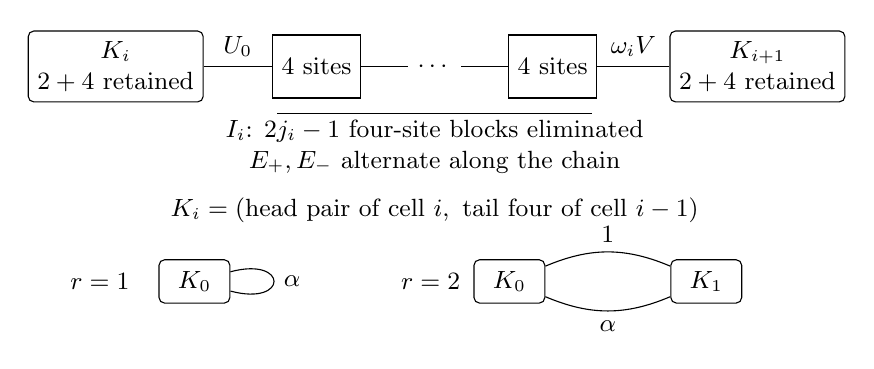
\begin{tikzpicture}[x=1cm,y=1cm,font=\small,
 core/.style={draw,rounded corners=2pt,minimum width=1.55cm,minimum height=.9cm,align=center},
 block/.style={draw,minimum width=1cm,minimum height=.8cm,align=center}]
\node[core] (kl) at (0,0) {$K_i$\\$2+4$ retained};
\node[block] (a) at (2.55,0) {$4$ sites};
\node (dots) at (4.05,0) {$\cdots$};
\node[block] (b) at (5.55,0) {$4$ sites};
\node[core] (kr) at (8.15,0) {$K_{i+1}$\\$2+4$ retained};
\draw (kl)--node[above] {$U_0$}(a);
\draw (a)--(dots); \draw (dots)--(b);
\draw (b)--node[above] {$\omega_i V$}(kr);
\draw (2.05,-.6)--(6.05,-.6);
\node[align=center] at (4.05,-1.02)
 {$I_i$: $2j_i-1$ four-site blocks eliminated\\$E_+,E_-$ alternate along the chain};
\node[align=center] at (4.05,-1.83)
 {$K_i=(\text{head pair of cell }i,\ \text{tail four of cell }i-1)$};
\node at (-.2,-2.73) {$r=1$};
\node[core,minimum width=.9cm,minimum height=.55cm] (one) at (1,-2.73) {$K_0$};
\draw (one) edge[loop right,looseness=8] node[right] {$\alpha$} (one);
\node at (4,-2.73) {$r=2$};
\node[core,minimum width=.9cm,minimum height=.55cm] (twoa) at (5,-2.73) {$K_0$};
\node[core,minimum width=.9cm,minimum height=.55cm] (twob) at (7.5,-2.73) {$K_1$};
\draw (twoa) to[bend left=23] node[above] {$1$} (twob);
\draw (twoa) to[bend right=23] node[below] {$\alpha$} (twob);
\end{tikzpicture}
\caption{Block couplings in $cI-A^2$, rather than individual graph edges.
The upper panel shows one interior chain when $j_i\ge2$; for $j_i=1$
it consists of one four-site block. The right coupling meets only the
tail-four slot of $K_{i+1}$. Eliminating all chains gives a cyclic matrix
on the $K_i$, with $\omega_i=1$ except $\omega_{r-1}=\alpha$.
The lower panels show the endpoint incidences when the cycle is a loop or
a pair of parallel chains: both contributions are added, and every core
has two incidences.}
\label{fig:boundary}
\end{figure}


\subsection{The additive cyclic Schur identity}

Use the same open pivot sequence as before and put
\[
 U_{a+1}=-U_aX_a^{-1}E_a.
\]
Equation~\eqref{eq:recurrence} gives $U_a=(R_a^T,W_a)^T$,
that is, the vertical stack of $R_a$ and $W_a^T$.
For the final interior index $p_i=2j_i-2$, define
\begin{equation}
 \mathcal L_i=\sum_{a=0}^{p_i}U_aX_a^{-1}U_a^T,
 \qquad \mathcal P_i=V^TX_{p_i}^{-1}V,
 \qquad F_i=U_{p_i}X_{p_i}^{-1}V.
 \label{eq:endpoint-data}
\end{equation}
Let $\iota_i:\R^6\to\R^{6r}$ be the coordinate embedding at $K_i$,
with the index $i+1$ understood cyclically.

\begin{lemma}[Exact cell assembly]\label{lem:assembly}
When the interior pivots are positive, their elimination gives the retained
matrix
\begin{align}
 \mathcal S={}&I_r\otimes\mathcal B
 -\sum_i\iota_i\mathcal L_i\iota_i^T
 -\sum_i\iota_{i+1}\mathcal P_i\iota_{i+1}^T\notag\\
 &-\sum_i\omega_i\bigl(
 \iota_iF_i\iota_{i+1}^T+\iota_{i+1}F_i^T\iota_i^T\bigr).
 \label{eq:assembly}
\end{align}
Every contribution is added, including coincident block locations when
$r=1$ or $r=2$.
\end{lemma}
\begin{proof}
At the current pivot of a chain, the left coupling is $U_a$, so the Schur
complement subtracts $U_aX_a^{-1}U_a^T$ from its retained left endpoint
and propagates the response as $-U_aX_a^{-1}E_a$.
Only the final pivot also sees the right endpoint, through $\omega_iV$.
Its two self-energy terms and cross term are precisely
\eqref{eq:endpoint-data}. Distinct interiors do not couple, so their
Schur contributions add.
For $r=2$, two different chains connect the same pair of retained cores;
both cross contributions remain in \eqref{eq:assembly}.
For $r=1$, the combined coupling at the final pivot is
$U_{p_0}+\omega_0V^T$. Expanding its quadratic Schur correction gives
$\mathcal P_0$ and the loop contribution
$\omega_0(F_0+F_0^T)$ in addition to $\mathcal L_0$.
Thus the same additive formula also covers the one-cell case.
\end{proof}

\subsection{The common limit and the degree-two estimate}

At either certified cap, suppose $p_i=J+2s_i$ with $s_i\ge0$, and put
$s=\min_i s_i$. Define
\[
 \mathcal L_\infty=\sum_{a\ge0}U_aX_a^{-1}U_a^T,
 \qquad \mathcal P_\infty=V^TX_*^{-1}V.
\]
By the stacked form of $U_a$, the matrix
$\mathcal B-\mathcal L_\infty-\mathcal P_\infty$ equals exactly
$S_\infty$ from \eqref{eq:Sinfty}. Its positivity has already been
proved; there is no new limiting-core assumption.

The separate response bounds give
\[
 \norm{U_{J+2v}}_2\le\sqrt2\,a q^v,
 \qquad \norm{U_{J+2v+1}}_2\le\sqrt2\,b q^v.
\]
Counting both increments in every pair therefore yields
\begin{equation}
 \norm{\mathcal L_\infty-\mathcal L_i}_2
 \le\frac{12b^2q^{2s_i}}{1-q^2}.
 \label{eq:Ltail}
\end{equation}
The right side harmlessly includes the final included term as well as
the actual suffix. The inverse identity and $\norm V_2\le\sqrt{14}$
give
\begin{equation}
 \norm{\mathcal P_i-\mathcal P_\infty}_2
 \le576\delta\theta^{s_i}.
 \label{eq:Ptail}
\end{equation}
Finally,
\begin{equation}
 \norm{F_i}_2\le3\sqrt{28}\,a q^{s_i}<16a q^{s_i}.
 \label{eq:Ftail}
\end{equation}

The diagonal part of \eqref{eq:assembly}, relative to
$I_r\otimes S_\infty$, combines one outgoing error from
\eqref{eq:Ltail} with one incoming error from \eqref{eq:Ptail}.
For the cross terms, take arbitrary $v_i\in\R^6$. Their quadratic form
has absolute value at most
\begin{align*}
 \sum_i2\norm{F_i}_2\norm{v_i}_2\norm{v_{i+1}}_2
 &\le\sum_i\norm{F_i}_2(\norm{v_i}_2^2+\norm{v_{i+1}}_2^2)\\
 &\le2\max_i\norm{F_i}_2\sum_i\norm{v_i}_2^2.
\end{align*}
Each retained core has exactly two chain-end incidences, counting a loop
twice and retaining both parallel contributions. This proves the bound
for every $r\ge1$, without summing an error $r$ times. We obtain
\begin{equation}
 \norm{\mathcal S-I_r\otimes S_\infty}_2
 \le E_s:=\frac{12b^2q^{2s}}{1-q^2}
              +576\delta\theta^s+32a q^s.
 \label{eq:assembly-error}
\end{equation}

\begin{proof}[Proof of Theorem~\ref{thm:cells}]
Exact arithmetic with the two parameter columns gives
\[
 E_0=
 \begin{cases}
 501647/468750000<1/500,&c=\czero,\\
 700000123/196875000000000000<10^{-8},&c=\cone.
 \end{cases}
\]
All terms in $E_s$ decrease with $s$. Proposition~\ref{prop:tail} already
supplies $S_\infty\succ(\gamma-\epsilon)I_6$, so
\eqref{eq:assembly-error} gives
\[
 \mathcal S\succ(\gamma-2\epsilon)I_{6r}\succ0.
\]
The condition $p_i=2j_i-2\ge J$ is exactly
$h_i\ge4(J+2)+2$, namely $106$ or $202$. All eliminated pivots are
positive by Section~\ref{sec:uniform}. Schur congruence now proves
$cI-A_N(\tau,\alpha)^2\succ0$, as required.
\end{proof}

The reduction is now uniform in both sources of variation: the shortest
cell controls the local tail, and two chain-end incidences at each retained
core control the global error. The full boundary matrix therefore remains
positive as the number of legal cells increases.

\section{Finite completion and explicit competitors}
\label{sec:finite}

The preceding analysis reduces each remaining statement to an explicitly
bounded set of rational positive-definiteness tests. We give the complete
ranges and the separating inequalities, including the cases where a
stronger proposed cap is false.

\subsection{The one-cell family and its uniform ceiling}

\begin{proof}[Proof of Theorem~\ref{thm:one-cell}]
For $k\ge25$, the single legal cell has length $8k+2\ge202$, so
Theorem~\ref{thm:cells} at $r=1$, $\alpha=+1$, and $c=\cone$ applies.
The remaining $k=1,\ldots,24$ are exactly the orders
\[
 10,18,26,\ldots,194.
\]
For each full signed graph the rational verifier proves
$\cone I-A_{8k+2}(w_k,+1)^2\succ0$ by positive scalar Schur pivots.
The $10\times10$ matrix is constructed and checked directly, without
assuming disjoint ordinary and wrap block locations. The first analytic
order is $202$, so no admissible size is missing.

At $c_-=7905369/1000000$ and order $202$, independent exact elimination
of $c_-I-A_{202}(w_{25},+1)^2$ has $196$ positive scalar interior pivots.
The retained six-coordinate core then has a strictly negative pivot after
a positive scalar-pivot prefix. The recorded rational pivot is strictly
negative, not merely nonpositive or a failed numerical test.
Schur congruence gives a vector with negative quadratic form, and hence
\[
 \rho(A_{202}(w_{25},+1))^2>c_-.
\]
This member supplies the lower endpoint in \eqref{eq:supremum}; the
uniform strict upper bounds supply the non-strict upper endpoint.
\end{proof}

\subsection{Two and three nearly equal legal cells}

For $r=2$ and $k\ge6$, the parameters
$\lfloor k/2\rfloor,\lceil k/2\rceil$ sum to $k$.
When $k\ge26$, each is at least $13$, so the cell bound $\czero$ applies.
Exactly twenty finite cases remain:
\begin{equation}
 k=6,\ldots,25,\qquad N=52,60,\ldots,204.
 \label{eq:R4finite}
\end{equation}
All use negative holonomy. For even $k$ their cell lengths are equal.
For odd $k$ the two lengths are $N/2-4$ and $N/2+4$, which changes the
placement from the older equally spaced gap construction. Each matrix in
\eqref{eq:R4finite} is rebuilt from its own word and passes exact rational
LDL positivity at cap $\czero$. The first analytic order is $212$.

For $r=3$, write $k=3q+s$, $0\le s<3$. The three parameters
\[
 \left\lfloor\frac{k}{3}\right\rfloor,
 \left\lfloor\frac{k+1}{3}\right\rfloor,
 \left\lfloor\frac{k+2}{3}\right\rfloor
\]
are $3-s$ copies of $q$ followed by $s$ copies of $q+1$.
They sum to $k$, are at least two for $k\ge6$, and differ by at most one.
For $k\ge39$ they are all at least thirteen, so Theorem~\ref{thm:cells}
applies with positive holonomy. The remaining thirty-three cases are
\begin{equation}
 k=6,\ldots,38,\qquad N=54,62,\ldots,310.
 \label{eq:R6finite}
\end{equation}
Each full signed graph passes exact rational LDL at cap $\czero$.
The first analytic order is $318$, immediately after the final admissible
finite order. When $3\nmid k$, the cells are nearly equal rather than
identical, and no certificate for another gap placement is substituted.

For both lists, the verification forms $(198/25)I-A^2$ or its
denominator-cleared equivalent $198I-25A^2$ directly from integer
two-edge walks. A separate implementation uses the normalized matrix and
a different scalar elimination order. For the three-cell list,
it also reconstructs the triangle signs independently from the
quadrilateral-gap word. Every required pivot in each list is strictly
positive. These are the only finite ranges left by the minimum-cell-length
reduction for the stated residue-four and residue-six families.

\subsection{The twisted comparison and the all-even witness range}

\begin{proof}[Proof of Theorem~\ref{thm:witnesses}]
For residue two, Theorem~\ref{thm:one-cell} gives the stronger cap
$\cone<\czero$ at every $k\ge6$. The two- and three-cell arguments above
give the cap $\czero$ for the other two residues.
For $x>0$, $\cos x>1-x^2/2$, and $\pi^2<10$. Therefore
\begin{equation}
 \tw(N)^2>8-\frac{20\pi^2}{N^2}>8-\frac{200}{N^2}.
 \label{eq:benchmark-lower}
\end{equation}
At $N\ge50$, the last expression is at least $198/25$.
Thus every nonzero residue witness satisfies
\eqref{eq:nonzero-witnesses}. In particular, the exact endpoint gaps for
the other two residues are
\[
 \frac{2679}{338}-\frac{198}{25}=\frac{51}{8450}>0,
 \qquad
 \frac{5782}{729}-\frac{198}{25}=\frac{208}{18225}>0,
\]
coming from $N=52$ and $N=54$ respectively.

For $N=8m\ge32$, Theorem~\ref{thm:period8} gives a witness with squared
radius at most $\etaedge$. The rational comparison
\begin{equation}
 \etaedge<\frac{999}{128}=8-\frac{200}{32^2}
 \label{eq:period8-separator}
\end{equation}
follows by squaring positive quantities: the intermediate bound is
\[
 \frac{(999/128-4)^2-10}{2}=\frac{73329}{32768}>\sqrt5,
 \quad 73329^2-5\cdot32768^2=8433121>0.
\]
Equations~\eqref{eq:benchmark-lower} and
\eqref{eq:period8-separator} prove the strict comparison at every such
order. The four residue classes now cover $32,40$ and every even $N\ge48$.
\end{proof}

\subsection{A stronger balanced subsequence and exact obstructions}

Equal cells admit one additional small-order completion.
\begin{proposition}\label{prop:balanced-sharp}
For every $j\ge1$,
\[
 \rho(A_{16j+4}(w_j\|w_j,-1))^2<\cone.
\]
For $j\ge3$ this value is strictly below the twisted benchmark.
\end{proposition}
\begin{proof}
Corollary~\ref{cor:phase} applies for $j\ge25$, with the two finite
phases $z=\pm\mathrm i$. The remaining $j=1,\ldots,24$, at orders
$20,36,\ldots,388$, have exact full-graph positive-definiteness certificates
for $790537I-100000A^2$. Both primary and independent rational replays
cover the complete list. Their smallest case uses a cell of length ten
and is checked directly, including the coincident couplings.
The first analytic order is $404$. For $j\ge3$, $N\ge52$, so
\eqref{eq:benchmark-lower} and $\cone<\czero$ give the comparison.
\end{proof}

The sharper cap cannot replace $\czero$ in the full residue-four theorem.
For the negative-holonomy nearly balanced words, exact rational elimination
gives
\begin{align*}
 \rho(A_{60}(w_3\|w_4,-1))^2&>\cone,\\
 \rho(A_{76}(w_4\|w_5,-1))^2&>\cone.
\end{align*}
In each case the certificate records a strictly negative pivot with its
complete positive predecessor prefix, proving a negative direction for
$\cone I-A^2$. Thus the obstruction is exact and applies to the actual
changed construction used here.
There is also a distinct obstruction for the older balanced $N=60$ gap
word $[6,4^6,6,4^6]$ with negative holonomy. Its half-length is thirty;
its triangle signs change sign under that half-shift rather than repeating
a legal $w_j$. It therefore lies outside
Proposition~\ref{prop:balanced-sharp}, and its own exact negative pivot
confirms that dropping the even-$k$ condition would be false.
None of these obstructions contradicts the $\czero$ bound or gives an
unrestricted lower bound over all signings.

\section{Verification, provenance, and remaining questions}
\label{sec:verification}

The proof has three exact computational inputs: the fixed rational
premises of Lemma~\ref{lem:finite-premises}, the explicitly bounded finite
graph lists, and the strict lower obstructions. Everything that extends
those data to unbounded lengths, phases, or numbers of cells is proved in
Sections~\ref{sec:uniform} and~\ref{sec:cells}.
The finite lists are summarized below; a separate seed check supplies each
long-cell argument.
\begin{center}
\small
\begin{tabular}{lccc}
\toprule
Family & Finite parameter range & Graph orders & Analytic from\\
\midrule
One cell ($\cone$) & $1\le k\le24$ & $10,18,\ldots,194$ & $202$\\
Two equal cells ($\cone$) & $1\le j\le24$ & $20,36,\ldots,388$ & $404$\\
Two near-equal cells ($\czero$) & $6\le k\le25$ & $52,60,\ldots,204$ & $212$\\
Three near-equal cells ($\czero$) & $6\le k\le38$ & $54,62,\ldots,310$ & $318$\\
\bottomrule
\end{tabular}
\end{center}

All acceptance comparisons use integers or rational numbers. Positive
pivots certify positive definiteness by exact Schur congruence; negative
pivots with positive predecessors certify the claimed strict obstructions.
The scripts store construction parameters, pivot counts, exact certificate
matrices or pivot data, and integrity digests. Digests identify outputs;
the mathematical tests are the rational computations that generate them.
Floating spectra used during exploration are excluded from the proof.

Independent replays reconstruct the underlying graphs or isolated chain
responses separately, use different elimination orderings where applicable,
and match the exact statements rather than trusting stored positivity flags.
For example, the unequal-cell replay compares direct full-graph elimination
with independently eliminated chains embedded additively into the cyclic
boundary space, including loops and parallel contributions. These finite
comparisons test the implementations; Lemma~\ref{lem:assembly} proves the
identity for every admissible length and number of cells.

\subsection{An immutable supplement and its entry points}

All proof inputs are available in the commit-pinned supplement
\cite{C029Supplement}. Its revision is
\nolinkurl{12e3389c07cc5a632023a1f6b972f9baf450a6a0}; both the
\href{https://github.com/whzy3185/math/tree/12e3389c07cc5a632023a1f6b972f9baf450a6a0/research/c029_holonomy_schur_20261005}{source tree}
and the \href{https://github.com/whzy3185/math/archive/12e3389c07cc5a632023a1f6b972f9baf450a6a0.zip}{downloadable repository archive}
are fixed to that revision. Within the archive, start in
\nolinkurl{research/c029_holonomy_schur_20261005/}.
The \href{https://github.com/whzy3185/math/blob/12e3389c07cc5a632023a1f6b972f9baf450a6a0/research/c029_holonomy_schur_20261005/README.md}{supplement README}
gives the producer and independent-replay commands in dependency order.
Reproducing the complete suite requires Python~3 and SymPy~1.14.0;
NumPy is optional and is not part of an acceptance predicate. In particular,
the analytic producer precedes its two direct-graph replays, and the
residue-six producer precedes its independent replay.

The following map identifies the proof inputs relative to that directory.
Running \texttt{python} followed by each listed verifier path regenerates
its exact output alongside the source.
\begin{enumerate}
\item Lemma~\ref{lem:finite-premises} at $\czero$:
\nolinkurl{certificates/analytic/verify_r2_certificate.py};
its direct-graph seed and local-response replays are in
\nolinkurl{certificates/audit/}.
\item Lemma~\ref{lem:finite-premises} at $\cone$,
Theorem~\ref{thm:one-cell}, and the order-$202$ lower obstruction:
\nolinkurl{certificates/strengthening/verify_uniform_cap.py}.
\item Proposition~\ref{prop:balanced-sharp} and the older order-$60$
obstruction: \nolinkurl{certificates/r4_pilot/verify_r4_pilot.py}.
\item Lemma~\ref{lem:assembly}, the near-equal two-cell list, and its
order-$60$ and order-$76$ obstructions:
\nolinkurl{certificates/unequal_cells/verify_unequal_cells.py},
with the additive construction in the same directory's
\nolinkurl{assembly.py}.
\item The three-cell finite list:
\nolinkurl{certificates/r6_completion/verify_r6_completion.py}.
\item The fiber determinant and the order-$32$ integer check:
\nolinkurl{certificates/new_conjecture/verify_antiperiodic_counterexample.py}.
\end{enumerate}
The four finite parameter lists are exactly those in the table above.
Each later certificate directory has its own \nolinkurl{audit/}
subdirectory; all four raw replay scripts are also included in the source
bundle accompanying this revision. Its reproduction instructions list every
producer and replay, including their dependencies. The accompanying
unequal-cell producer explicitly requires the order-$60$ and order-$76$
strict obstructions and records their complete pivot prefixes; this is a
checker refinement relative to the pinned archive. Both obstructions are
also required by the independent assembly replay already in that archive.
The mathematical assertions and frozen proof inputs are unchanged.

\subsection{The frozen formal statement}

A separate Lean development verifies the exact negative-holonomy finite
radius in Theorem~\ref{thm:period8}. For the explicit raw graph matrix and
every positive cell count, it proves that all Hermitian eigenvalue moduli
are at most the stated radical and that an eigenvalue equals its positive
value. The proof includes the seam and raw-operator bridges, maximal
antiperiodic phase, determinant root, and lower attainment. The formal scope cited here is specifically the
\href{https://github.com/whzy3185/math/tree/12e3389c07cc5a632023a1f6b972f9baf450a6a0/research/c029_holonomy_schur_20261005/lean/exact_radius}{\texttt{lean/exact\_radius/} subbundle}
of the pinned supplement, verified on 5 October 2026. It freezes the
$237$-declaration Lean~4.33.1 audit with axiom union exactly
\texttt{propext}, \texttt{Classical.choice}, and \texttt{Quot.sound}.
This count refers to that subbundle, not to subsequent addenda present in
the repository. Its \nolinkurl{reproduction/} directory fixes the toolchain
and dependency manifest, including Mathlib commit
\nolinkurl{0df444a360eaa60ab8c11dca51a86af692955474}.
The supplied patch applies to baseline commit
\nolinkurl{7b6a351cc5f8f83f5527b7fc547f0a865ea50cf2}.
From the resulting \nolinkurl{formal/} directory, run these commands in order:
\begin{quote}\small\ttfamily
lake build TargetA.Period8ExactFiniteRadius\\
lake env lean ExactRadiusAxiomAudit.lean
\end{quote}

\begin{samepage}
The final declarations in \nolinkurl{TargetA/Period8ExactFiniteRadius.lean}
are \nolinkurl{TargetA.period8_alpha_minus_exact_finite_radius} for the
upper bound and equality in the raw graph's Hermitian eigenvalue list,
\nolinkurl{TargetA.period8_alpha_minus_finite_radius_attained_index} for
positive attainment, and \nolinkurl{TargetA.period8_finite_radius_radical}
for the displayed radical. The subbundle includes their full sources,
build and axiom-audit logs, source hashes, and verification summary.
\par\end{samepage}

The separate quartic identification used to name the conjectured constant,
the finite-size asymptotic, the integer principal-minor certificate, and
the Riccati/Schur and residue-completion arguments are not formalized by
that checkpoint. They retain their stated analytic and exact-certificate
evidence.

\subsection{Provenance and remaining questions}

The exact period-eight formula and the witness range are inherited
project results; the present application to the revised conjecture and the
common unequal-cell proof have their scope distinguished in the supplement's
claim ledger. The new proof requires neither the older physical
interface-edge calculation nor an IMS localization estimate or a count of
localized modes. It does not change the status of historical equality
certificates at smaller orders.

The principal extremal problem remains to determine $\mu_N$ and its
minimizing switching classes. Even within the prescribed one-cell family,
the interval \eqref{eq:supremum} does not determine the exact supremum or
prove convergence. For broader cell arrangements, the two-cell
obstructions at orders $60$ and $76$ show that shortening cells can affect
the sharper cap. A structural lower bound over arbitrary triangle-sign
words would be needed to turn any of these explicit upper bounds into a
global minimization theorem.


\begin{thebibliography}{9}
\small
\bibitem{Suvagiya2026old}
V. Suvagiya,
\emph{Signed circulants at the Ramanujan bound},
arXiv:2607.18334v1, 19 July 2026;
withdrawn in version 2, 22 September 2026, and merged into
\cite{Suvagiya2026}.
\url{https://arxiv.org/abs/2607.18334}.

\bibitem{Suvagiya2026}
V. Suvagiya,
\emph{Parity families and signed spectra: kernel averaging,
near-Ramanujan bounds, and exact circulant models},
arXiv:2607.17343v2, 22 September 2026,
Theorem 26, Remark 27, and Conjecture 28.
\url{https://arxiv.org/abs/2607.17343v2}.

\bibitem{LuoRoy2026}
Y. Luo and A. Roy,
\emph{Homological spectral graph theory and weighted cycle counting},
arXiv:2403.01550v4, 4 August 2026.
\url{https://arxiv.org/abs/2403.01550v4}.

\bibitem{ChenDamBu2024}
L. Chen, E. R. van Dam, and C. Bu,
Spectra of power hypergraphs and signed graphs via parity-closed walks,
\emph{Journal of Combinatorial Theory, Series A} \textbf{207} (2024),
105909.
\url{https://doi.org/10.1016/j.jcta.2024.105909}.

\bibitem{EarlierPeriodEight}
Y. Zhao and J. Li,
\emph{Half-Cell Flux and an Exactly Solvable Period-Eight Phase in Signed
Cycle Squares}, unpublished project manuscript, Section 4,
repository snapshot of 14 September 2026, commit
\nolinkurl{085ea698475b7b32e0ae57457ec903a922248f69}.
\href{https://github.com/whzy3185/math/blob/085ea698475b7b32e0ae57457ec903a922248f69/research/paper_strengthening/manuscript_period8_jgt/frontmatter_en.tex}{Title and author record};
\href{https://github.com/whzy3185/math/blob/085ea698475b7b32e0ae57457ec903a922248f69/research/paper_strengthening/manuscript_period8_jgt/sections_en/04_period8_exact.tex}{exact period-eight source}.

\bibitem{EarlierTargetA}
\texttt{whzy3185/math} project,
\emph{Finite Structured Counterexample Tail}, unpublished Target A
proof package (no author line in the source), repository snapshot of
1 September 2026, commit
\nolinkurl{44ff33a89294056907d0b909d68a8db27371c4f0}.
\href{https://github.com/whzy3185/math/blob/44ff33a89294056907d0b909d68a8db27371c4f0/research/proofs/task54/TARGET_A_FINITE_STRUCTURED_COUNTEREXAMPLE_TAIL.md}{Frozen construction and finite-tail source}.

\bibitem{C029Supplement}
\texttt{whzy3185/math} project,
\emph{C029: holonomy and Schur-tail research increment},
reproducibility supplement, 5 October 2026, commit
\nolinkurl{12e3389c07cc5a632023a1f6b972f9baf450a6a0}.
\href{https://github.com/whzy3185/math/tree/12e3389c07cc5a632023a1f6b972f9baf450a6a0/research/c029_holonomy_schur_20261005}{Frozen supplement};
\href{https://github.com/whzy3185/math/archive/12e3389c07cc5a632023a1f6b972f9baf450a6a0.zip}{repository archive at the same commit}.

\bibitem{BelardoBrunetti2024}
F. Belardo and M. Brunetti,
Limit points for the spectral radii of signed graphs,
\emph{Discrete Mathematics} \textbf{347}(2) (2024), 113745.
\url{https://doi.org/10.1016/j.disc.2023.113745}.

\bibitem{KannanPragada2023}
M. R. Kannan and S. Pragada,
Signed spectral Tur\'an type theorems,
\emph{Linear Algebra and its Applications} \textbf{663} (2023), 62--79.
\url{https://doi.org/10.1016/j.laa.2023.01.002}.
\href{https://arxiv.org/abs/2204.09870v3}{Author preprint, version 3}.

\end{thebibliography}
\end{document}
